\section{Preliminaries}


\begin{frame}\frametitle{Compressive Sensing 1/2}
Candes \& Donoho による信号や画像の低次元表現の枠組み
\begin{equation}
    f = \Phi x \; (\Phi: N \times N, x: N \times 1)
\end{equation}
$x$ 中で $K$ 個の係数しか大きな値を取らないとき,$x$ を $f$ の $K$ 疎表現と呼ぶ.
\begin{eqnarray}
    y & = & \Omega f = \Theta x \; (\Omega: M \times N, y: M \times 1) \\
    \Theta & = & \Omega \Phi
\end{eqnarray}
上記の低次元空間への射影 $\Theta$ を sensing matrix と呼ぶ.
$\Theta$ は Ristricted Isometry Property
\begin{eqnarray}
    (1 - \delta_k) ||c||^2_2 \leq & || \Theta_c ||^2_2 & \leq (1 + \delta_k) ||c||^2_2 \\
    0 < & \delta_k & < 1
\end{eqnarray}
を満たすとする,ただし $c$ はランダムな $K$ 疎ベクトルである.
\end{frame}


\begin{frame}\frametitle{Compressive Sensing 2/2}
最適な疎表現 $x$ の導出は$L_0$最適化問題だが NP 困難なので,次の $L_1$ ノルム最適化に近似
\begin{equation}
    \arg\min ||x||_1 \; s.t. \; y = \Theta x
\end{equation}
\begin{block}{主な最適化アルゴリズム}
\begin{itemize}
    \item 貪欲法\\
        Match Pursuit (MP),
        Orthogonal MP (OMP)\footnote{筆者らは OMP を採用 (scikit-learn など多くのライブラリでも標準)}

    \item 凸緩和最適化\\
        Gradient Projection for Sparse Reconstruction (GPSR),\\
        Total Variation (TV),
        Smoothed-$L_0$ (S$L_0$)
\end{itemize}
\end{block}
\end{frame}


\begin{frame}\frametitle{K-SVD の位置づけ}
compressive sensing と行列因子分解法
\end{frame}


\begin{frame}\frametitle{K-SVD の定式化}
\label{ksvd}

訓練データセット $\{ x \}$ から疎な辞書 $D$ (= sensing matrix)を構築できるアルゴリズム.
最適化問題としての定式化は以下
\begin{eqnarray}
    \min \{||x||_0\} &s.t.& \min ||Y-DX||^2_F \leq \varepsilon \; (i = 1, \dots, N) \\
    ||Y-DX||^2_F &=& ||Y - \sum D_k x_k||^2_F \\
    &=& ||(Y - \sum_{k \neq j} d_k x_k) - d_j x_j||^2_F \\
    &=& ||E_j - d_j x_j||^2_F
\end{eqnarray}
ただし$||\cdot||_F$ はフロベニスノルム $||A||_F = \sqrt{\sum{A^2_{i,j}}}$
\end{frame}


\begin{frame}\frametitle{K-SVD + OMP 更新アルゴリズム}
\end{frame}


\begin{frame}{Singular Value Decomposition}
\end{frame}



\begin{frame}\frametitle{Morphological image processing}
\begin{block}{Morphology}
特徴量抽出の前・後処理によく用いられる.主に以下の2種類
\begin{itemize}
    \item Dilation - 孤立点の除去
    \item Erosion - 欠落点の穴埋め
\end{itemize}
\end{block}

イメージ図\footnote
{\url{http://jp.mathworks.com/help/images/morphology-fundamentals-dilation-and-erosion.html}}
:実際は円状の構造要素(図中灰色)を利用
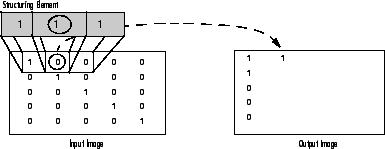
\includegraphics[scale=0.4]{figure/morph.png}
\end{frame}
